% Chapter 2: Diagrama Entidad Relación (DER)
	\chapter{Diagrama Entidad Relación (DER)}\label{Chap: DER}
	A continuación se muestra el Diagrama Entidad Relación (DER) del proceso que sigue el restaurante.

	\begin{figure}[h!]
		\centering
		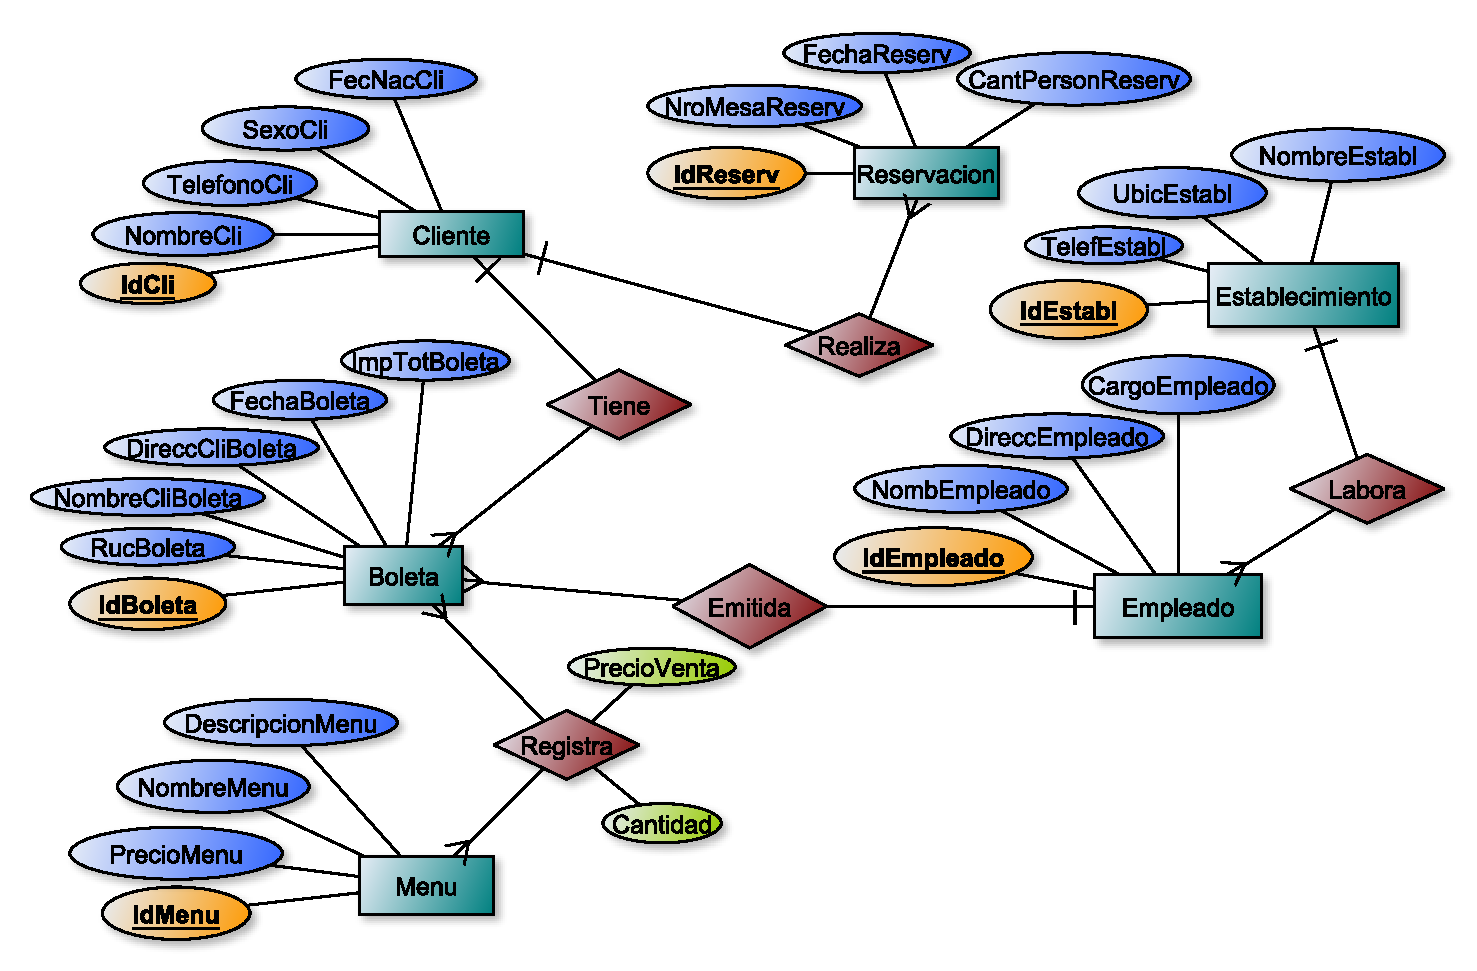
\includegraphics[scale = 0.6]{DER.pdf}
		\caption{Diagrama Entidad Relación (DER) de un Restaurante}
		\label{fig: DER Restaurante}
	\end{figure}
	
   La lectura del diagrama es lo siguiente: un cliente puede realizar muchas reservaciones y una reservación puede ser realizado solamente por un cliente; un cliente puede tener muchas boletas y una boleta le pertenece solamente a un cliente; una boleta puede ser emitido por un empleado y un empleado puede emitir muchas boletas; un empleado labora solamente en un establecimiento y en un establecimiento laboran muchos empleados; una boleta puede registrar muchos menús y un menú se puede registrar en muchas boletas.
	
	
	
	
	